\section{極値点探索の手法} % 三章
\label{sec:extremum_search}
  Remesのアルゴリズムの各ステップにおいて，現在の誤差関数 $E(x) = f(x) - P(x)$ の極値（最大値および最小値）を与える点 $x$ を高精度に特定することは，近似多項式の収束性を左右する重要な工程である．通常,グリッドを細かくすることで極値を精密に導出することができるが，計算コストが高くなるという欠点がある．
  誤差関数は近似が進むにつれて等振動性を示し，極値付近での挙動が非常に平坦になるため，数値微分を用いるニュートン法などは桁落ち誤差の影響を受けやすくなる．
  対策として二次関数補間を行う手法を思いついたが調べているうちに，導関数を用いずに高い収束速度と大域的な収束保証を両立するBrent法というものがあったので紹介する．

  \subsection{Brent法のアルゴリズム構成}
  \label{subsec:brent_algorithm}
    Brent法は，収束が遅いが確実な黄金分割探索と，収束が速い逐次放物線補間を，関数の挙動に応じて動的に切り替えるハイブリッドアルゴリズムである．
    本手法は，極値が存在する区間を常に維持し，以下の状態変数を用いて探索を進める．
    基本的なアルゴリズムとしては競技プログラミングなどで用いられる黄金分割法を主として条件を満たしたときに限り放物線補間を行うというものである．

    \begin{itemize}
      \item $x$: 現在の最小値（または最大値）を与える最良点．
      \item $w$: 2番目に良い関数値を与える点．
      \item $v$: 3番目に良い関数値を与える点（または直前の $w$）．
      \item $u$: 新たに評価を行う試行点．
      \item $e$: 直前のステップ幅．
      \item $d$: 現在のステップ幅．
      \item $a^*$: 探索区間の左端．
      \item $b^*$: 探索区間の右端．
    \end{itemize}

    放物線補間を行うには3点が必要となるため，アルゴリズムは常に $(x, w, v)$ の3点を保持・更新し続ける．

  \subsection{放物線補間と更新変数の定義}
  \label{subsec:parabolic_interpolation}
    3点 $(x, f(x)), (w, f(w)), (v, f(v))$ を通る放物線の頂点として求められる試行点の変位 $d$ は，ラグランジュ補間の公式より次式で計算される．
    \begin{equation}
      \label{eq:parabolic_step}
      d = - \frac{1}{2} \frac{(x-w)^2 \{f(x)-f(v)\} - (x-v)^2 \{f(x)-f(w)\}}{(x-w)\{f(x)-f(v)\} - (x-v)\{f(x)-f(w)\}}.
    \end{equation}
    本アルゴリズムでは，数値的な安定性を確保するために，実際に $u = x + d$ を更新する前に，この $d$と $e$を用いた審査を行う．

  \label{subsec:bisection_condition}
  \subsection{強制二分条件～放物線近似,黄金比分割どっちを使うのか判定～}
    放物線補間は，関数が滑らかな場合には超一次収束（収束次数 $r \approx 1．3247$）を達成するが，関数の形状によっては解から遠ざかる（発散する）リスクがある．
    Brent法の特徴は，放物線補間によって提案されたステップ $d$ を無条件に採用せず，以下の「強制二分条件」によってその妥当性を検証する点にある．

    変数 $e$ を「2ステップ前の移動量」とする．今回の放物線補間によるステップ $d$ が採用されるためには，以下の不等式条件を満たさなければならない．
    \begin{equation}
      |d| < \frac{1}{2} |e|.
    \end{equation}
    この条件は，「放物線補間を適用し続けるならば，ステップ幅は2回の反復ごとに少なくとも半分以下に縮小しなければならない」ということを表している．
    
    もしこの条件が満たされない場合，あるいは計算された $u$ が区間 $[a, b]$ の端点に近すぎる場合，放物線補間は「収束が停滞している」あるいは「不安定である」と判断され，却下される．
    その代わりとして，より安全な黄金分割探索によるステップが採用される．
    \begin{equation}
      u = x + K \cdot (x \text{ から遠い方の区間端点までの距離}).
    \end{equation}
    ここで $K = \frac{3-\sqrt{5}}{2} \approx 0．382$ である．
    
    このメカニズムにより，Remesアルゴリズムの初期段階のように誤差関数の形状が乱れている場合でも，Brent法は黄金分割探索と同等の確実性で極値を追い込み，収束が進むにつれて自動的に放物線補間へ移行して高速に解に到達する．本実装において，許容誤差 $\texttt{tol}$ は機械イプシロン $\varepsilon$ を考慮して $\sqrt{\varepsilon}$ のオーダー（倍精度で約 $10^{-8}$）に設定した．

    ここで定数 $K$ の値は，探索区間の比率を一定に保つ黄金比 $\phi$ に由来する．
    区間を $1 : \phi$ （ただし $\phi = \frac{1+\sqrt{5}}{2}$）の比率で分割するとき，次のステップでも分割比率を維持するためには，内分点までの距離の比 $\rho$ が方程式 $\rho^2 + \rho - 1 = 0$ を満たす必要がある．
    この正の解は $\rho = \frac{\sqrt{5}-1}{2} \approx 0．618$ となり，これは $1/\phi$ に等しい．
    Brent法において，区間の端点から新しい試行点までの距離の割合 $K$ は，残りの区間の割合に相当するため，
    \begin{equation}
      K = 1 - \rho = 1 - \frac{\sqrt{5}-1}{2} = \frac{3-\sqrt{5}}{2} \approx 0．382
    \end{equation}
    として導出される\cite{brent-original}．

  \newpage  %% 改ページ ==================================================
  % =========================================================
  % Goプログラム (brent-plot.go) が生成した
  % プロセス可視化ファイル（グラフと表）を読み込む
  % =========================================================
  % Brent法のアルゴリズム図示と収束過程
\subsection{アルゴリズムの図示}
  \begin{figure}[H]
    \centering
    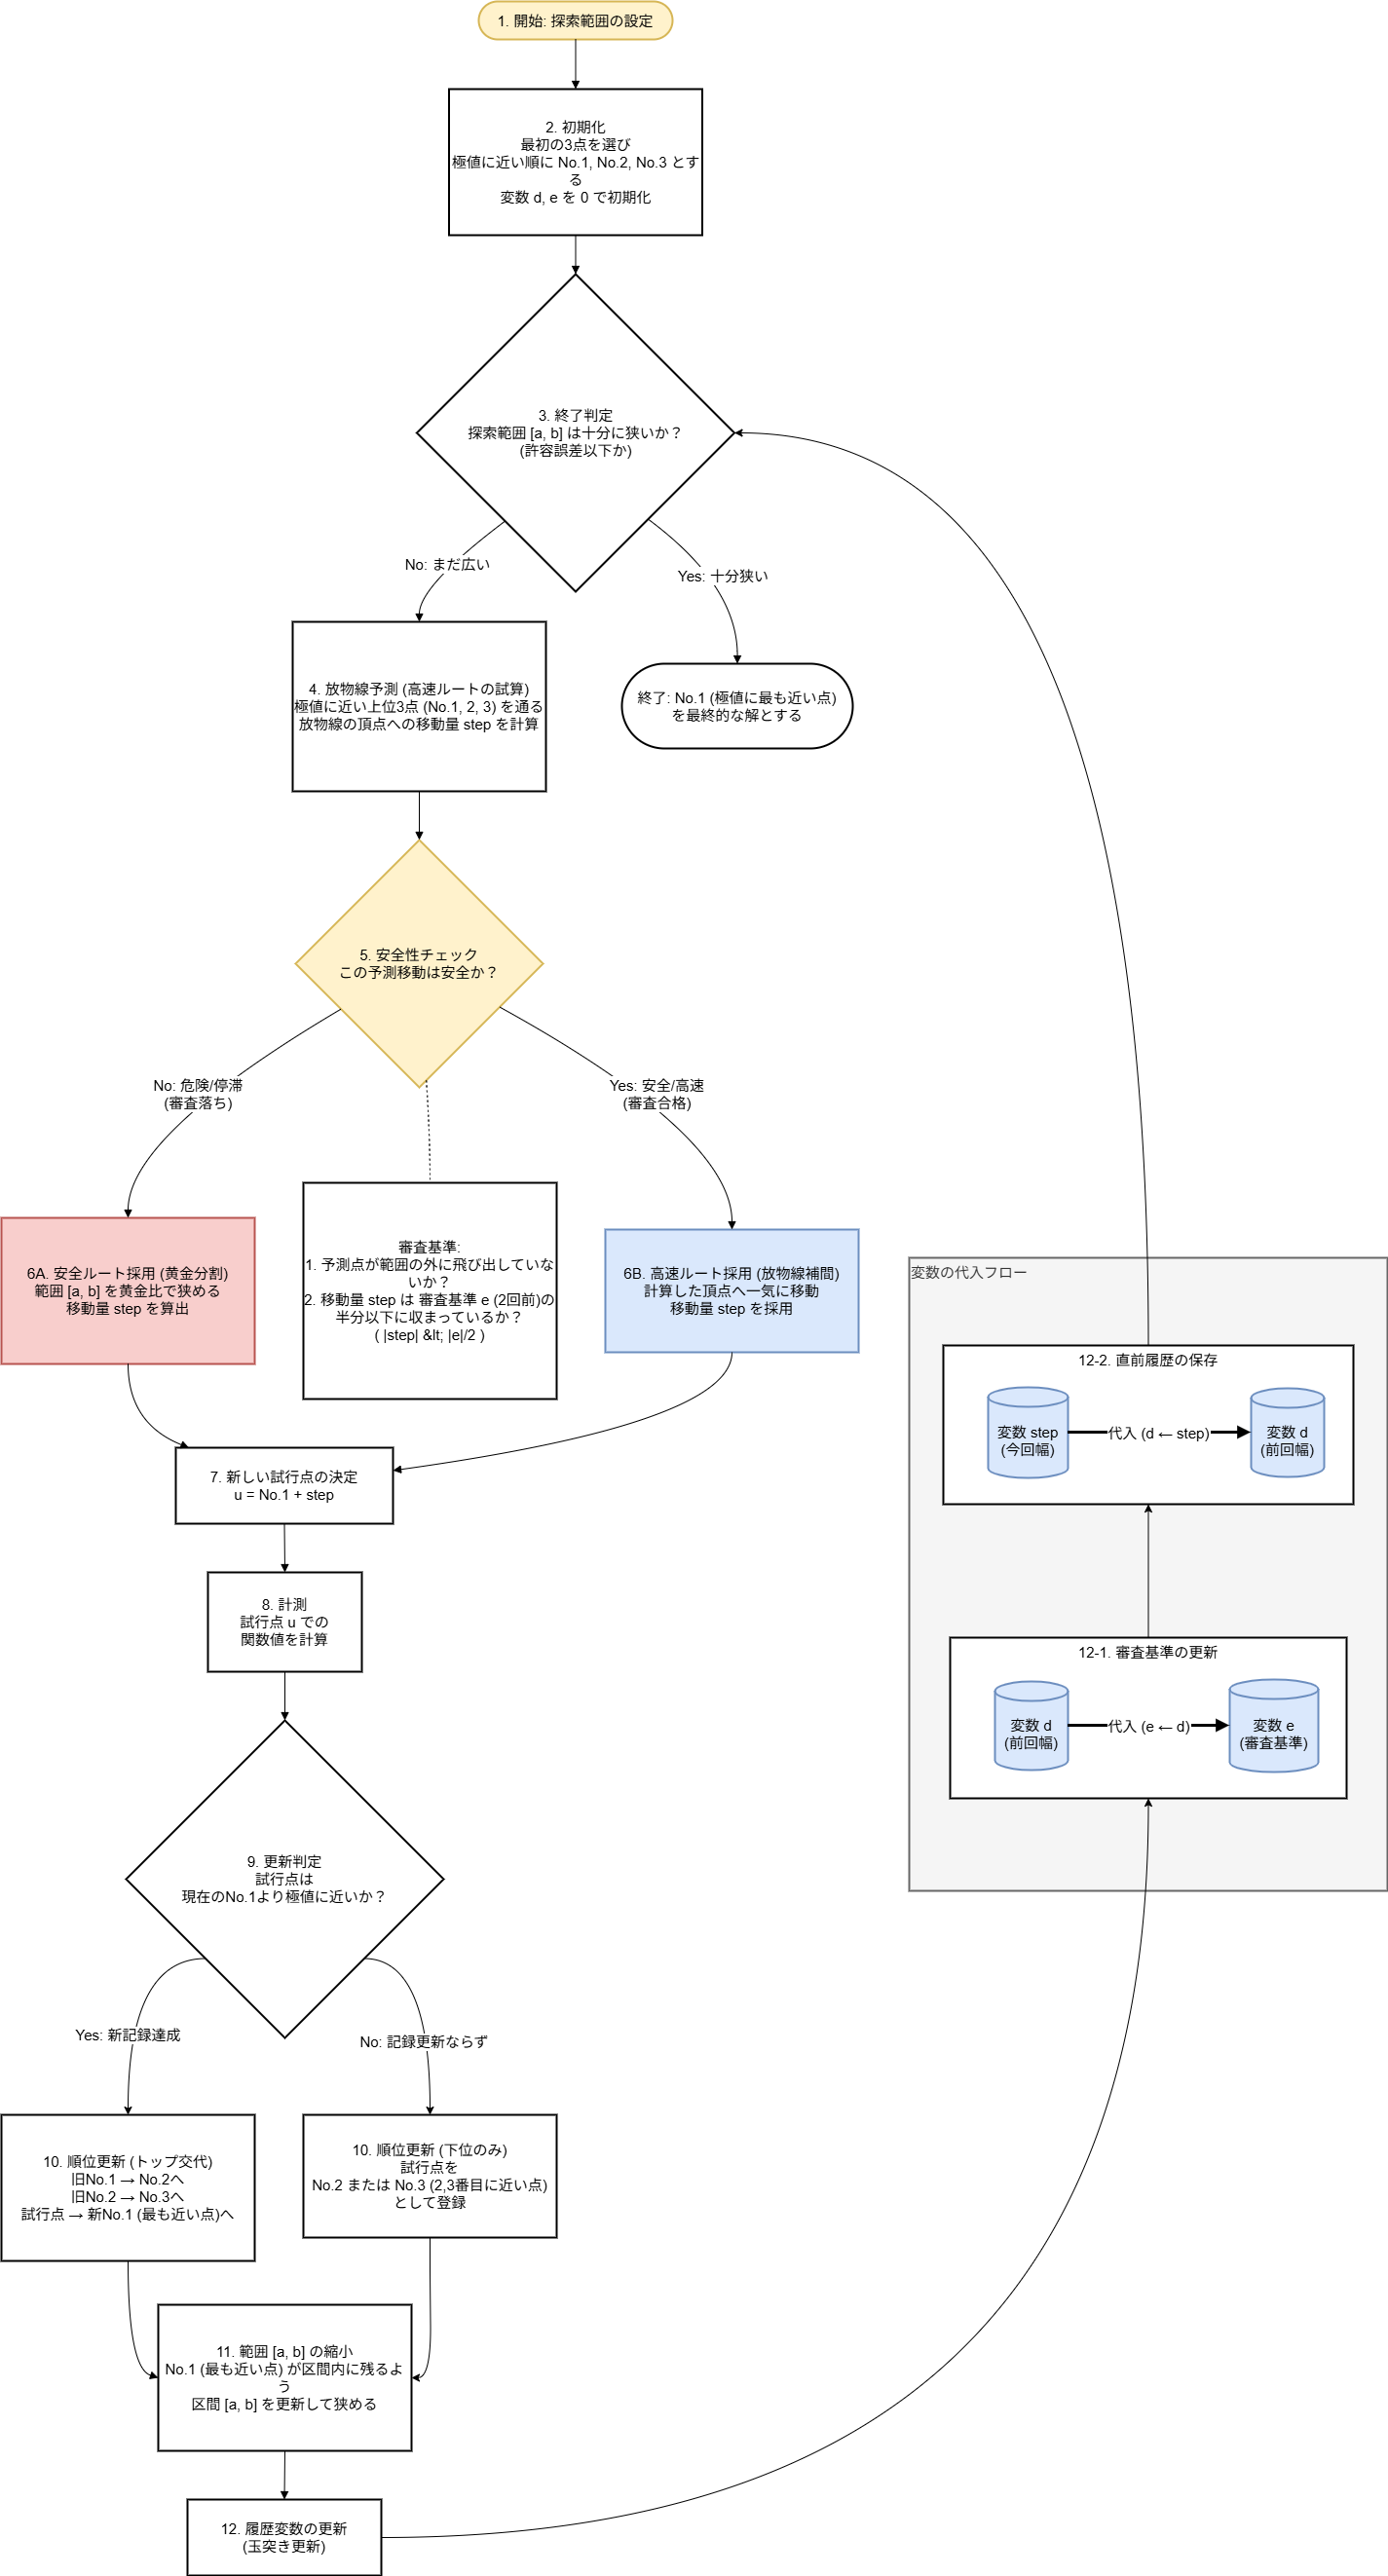
\includegraphics[width=0.7\linewidth]{material/brent/brent-architecture.png}
    \caption{Brent法のアルゴリズム構成}
  \end{figure}

\subsection{収束の様子}
  \begin{figure}[H]
    \begin{minipage}[b]{0.48\linewidth}
      \centering
      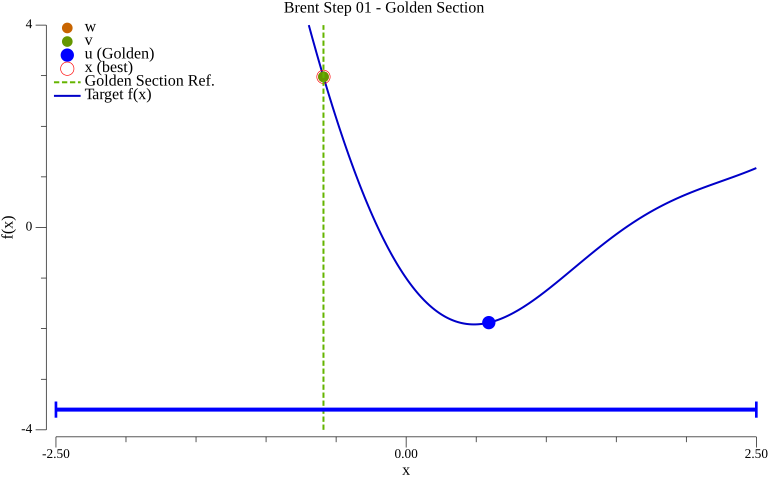
\includegraphics[width=1.0\linewidth]{material/brent/brent-step-01.png}
      \caption{Brent法-01回目}
    \end{minipage}
    \hfill
    \begin{minipage}[b]{0.48\linewidth}
      \centering
      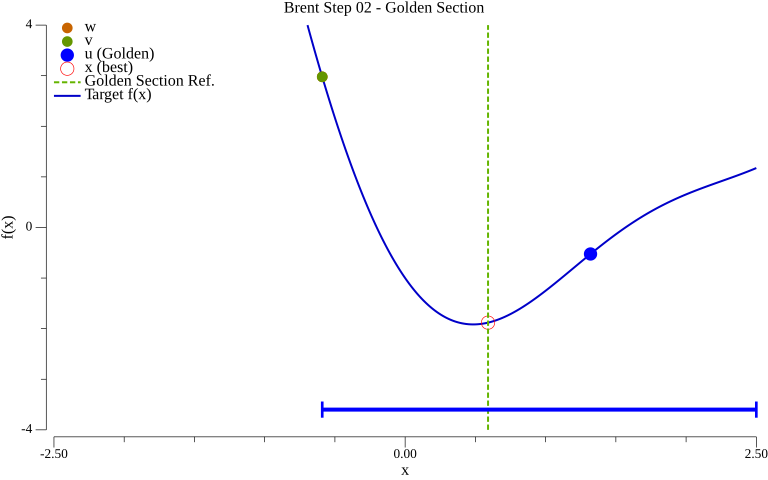
\includegraphics[width=1.0\linewidth]{material/brent/brent-step-02.png}
      \caption{Brent法-02回目}
    \end{minipage}
  \end{figure}
  \begin{figure}[H]
    \begin{minipage}[b]{0.48\linewidth}
      \centering
      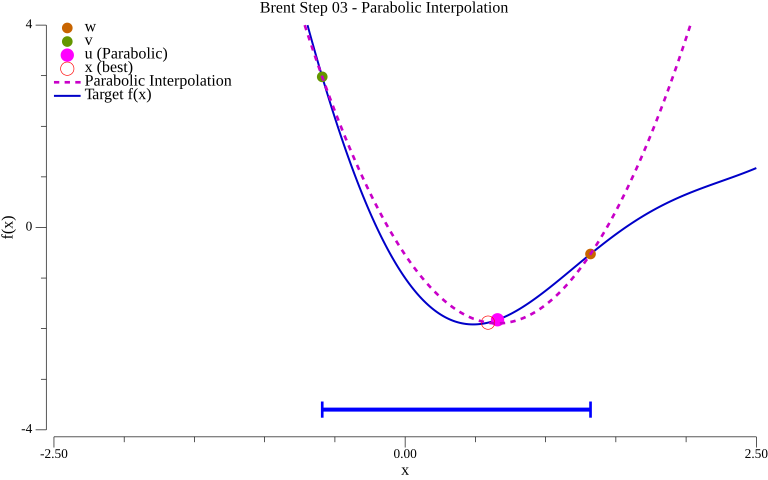
\includegraphics[width=1.0\linewidth]{material/brent/brent-step-03.png}
      \caption{Brent法-03回目}
    \end{minipage}
    \hfill
    \begin{minipage}[b]{0.48\linewidth}
      \centering
      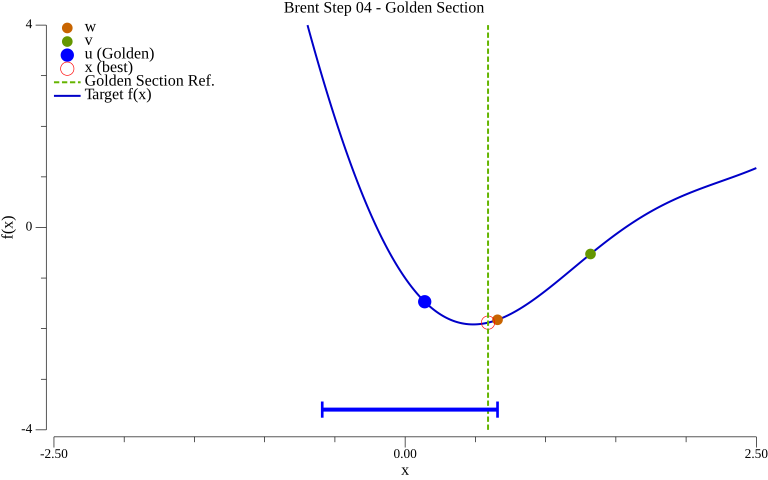
\includegraphics[width=1.0\linewidth]{material/brent/brent-step-04.png}
      \caption{Brent法-04回目}
    \end{minipage}
  \end{figure}
  \begin{figure}[H]
    \begin{minipage}[b]{0.48\linewidth}
      \centering
      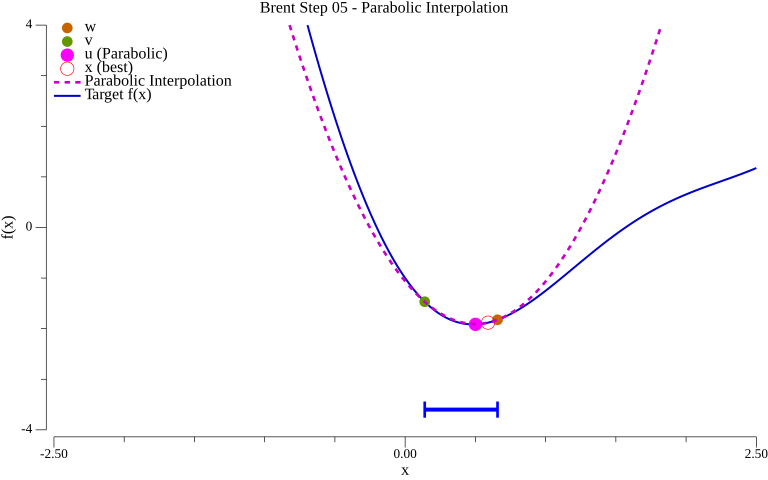
\includegraphics[width=1.0\linewidth]{material/brent/brent-step-05.png}
      \caption{Brent法-05回目}
    \end{minipage}
    \hfill
    \begin{minipage}[b]{0.48\linewidth}
      \centering
      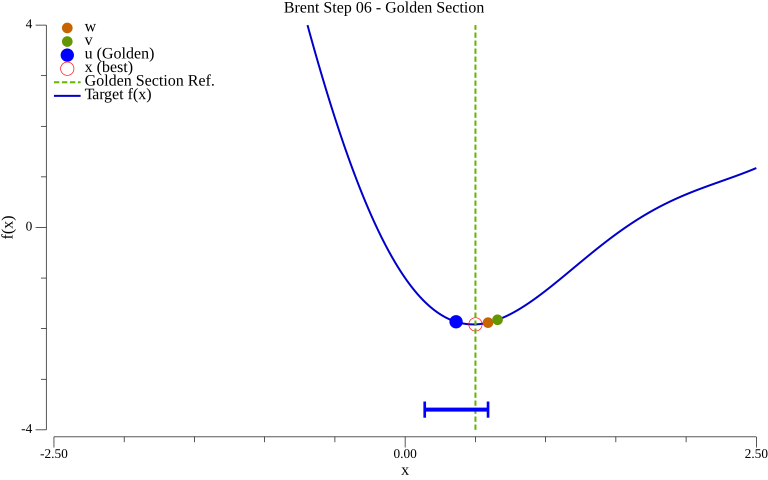
\includegraphics[width=1.0\linewidth]{material/brent/brent-step-06.png}
      \caption{Brent法-06回目}
    \end{minipage}
  \end{figure}
  \begin{figure}[H]
    \begin{minipage}[b]{0.48\linewidth}
      \centering
      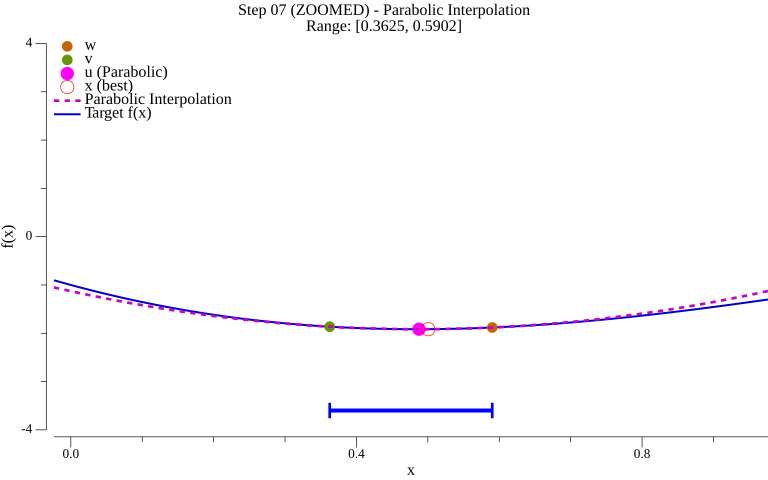
\includegraphics[width=1.0\linewidth]{material/brent/brent-step-07.png}
      \caption{Brent法-07回目}
    \end{minipage}
    \hfill
    \begin{minipage}[b]{0.48\linewidth}
      \centering
      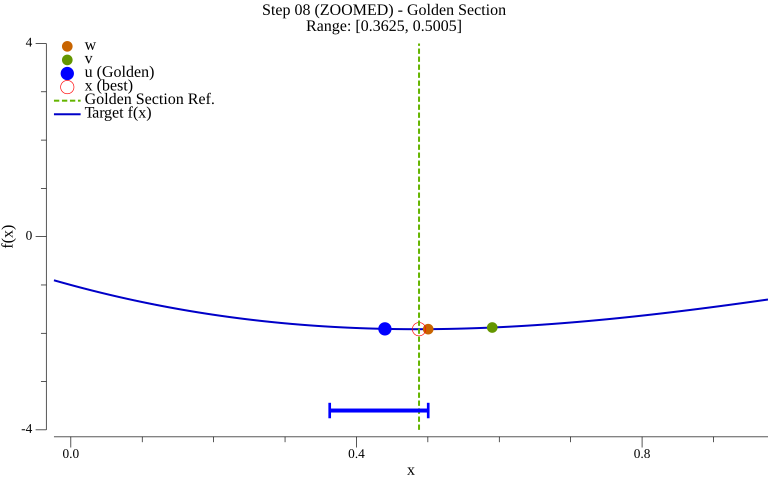
\includegraphics[width=1.0\linewidth]{material/brent/brent-step-08.png}
      \caption{Brent法-08回目}
    \end{minipage}
  \end{figure}
  \begin{figure}[H]
    \begin{minipage}[b]{0.48\linewidth}
      \centering
      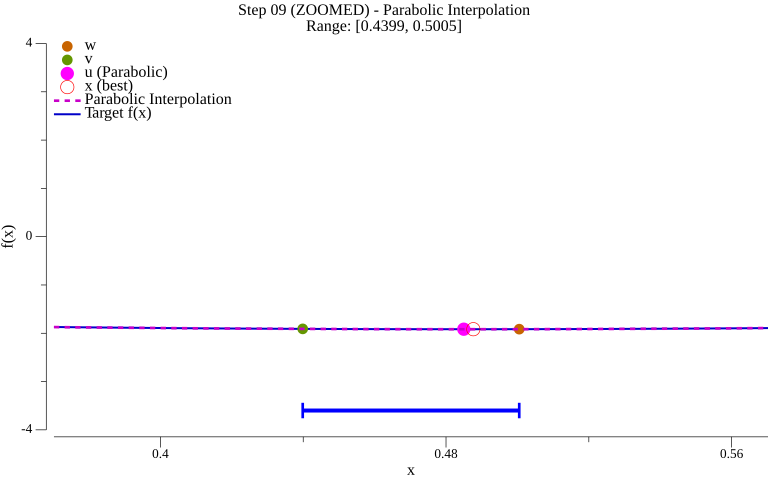
\includegraphics[width=1.0\linewidth]{material/brent/brent-step-09.png}
      \caption{Brent法-09回目}
    \end{minipage}
    \hfill
    \begin{minipage}[b]{0.48\linewidth}
      \centering
      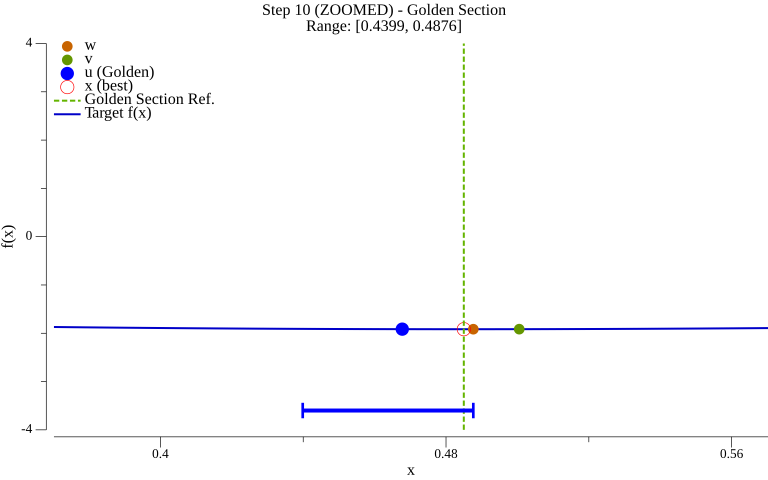
\includegraphics[width=1.0\linewidth]{material/brent/brent-step-10.png}
      \caption{Brent法-10回目}
    \end{minipage}
  \end{figure}
  \begin{figure}[H]
    \begin{minipage}[b]{0.48\linewidth}
      \centering
      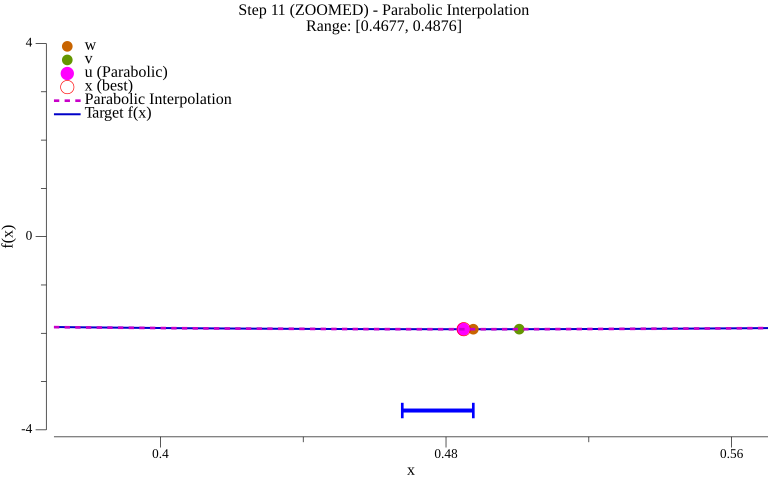
\includegraphics[width=1.0\linewidth]{material/brent/brent-step-11.png}
      \caption{Brent法-11回目}
    \end{minipage}
    \hfill
    \begin{minipage}[b]{0.48\linewidth}
      \centering
      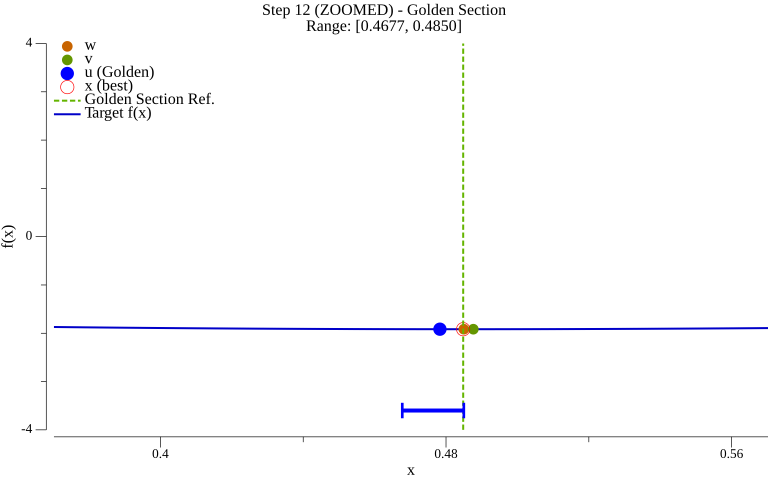
\includegraphics[width=1.0\linewidth]{material/brent/brent-step-12.png}
      \caption{Brent法-12回目}
    \end{minipage}
  \end{figure}
  \begin{figure}[H]
    \begin{minipage}[b]{0.48\linewidth}
      \centering
      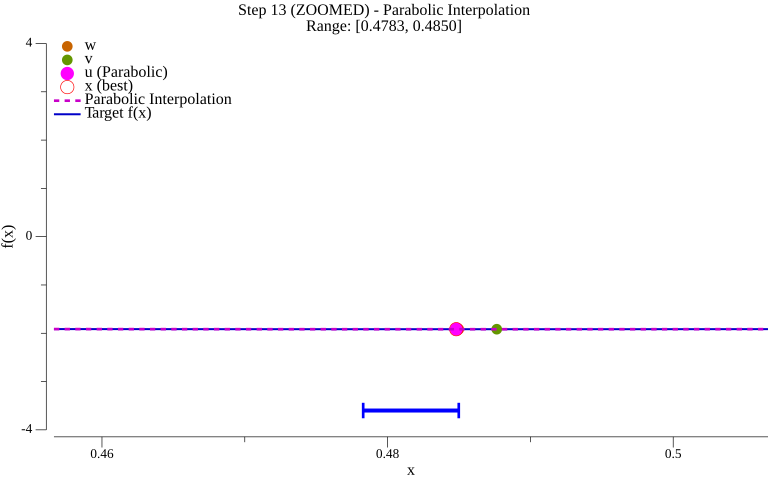
\includegraphics[width=1.0\linewidth]{material/brent/brent-step-13.png}
      \caption{Brent法-13回目}
    \end{minipage}
    \hfill
    \begin{minipage}[b]{0.48\linewidth}
      \centering
      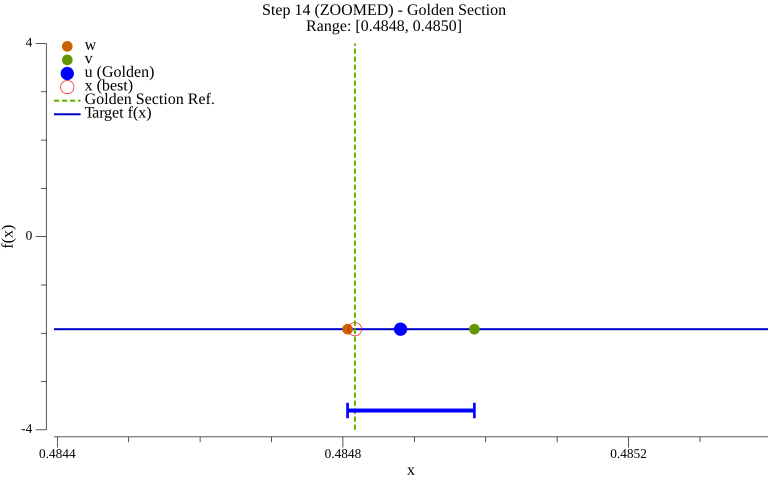
\includegraphics[width=1.0\linewidth]{material/brent/brent-step-14.png}
      \caption{Brent法-14回目}
    \end{minipage}
  \end{figure}
  \begin{figure}[H]
    \begin{minipage}[b]{0.48\linewidth}
      \centering
      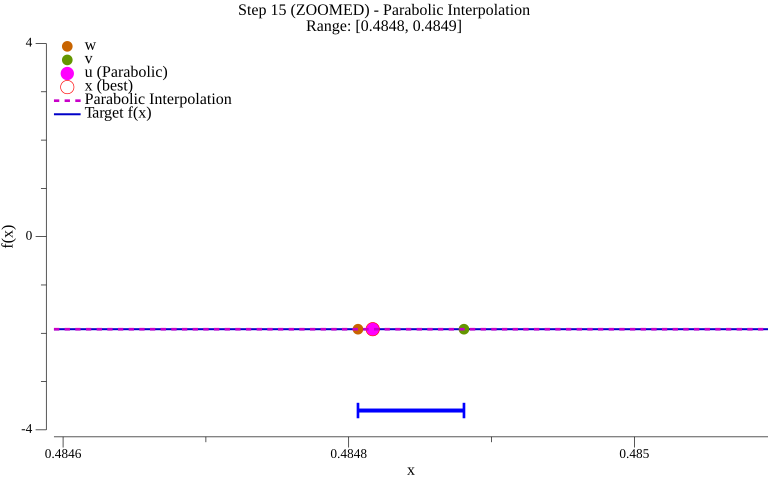
\includegraphics[width=1.0\linewidth]{material/brent/brent-step-15.png}
      \caption{Brent法-15回目}
    \end{minipage}
    \hfill
    \begin{minipage}[b]{0.48\linewidth}
      \centering
      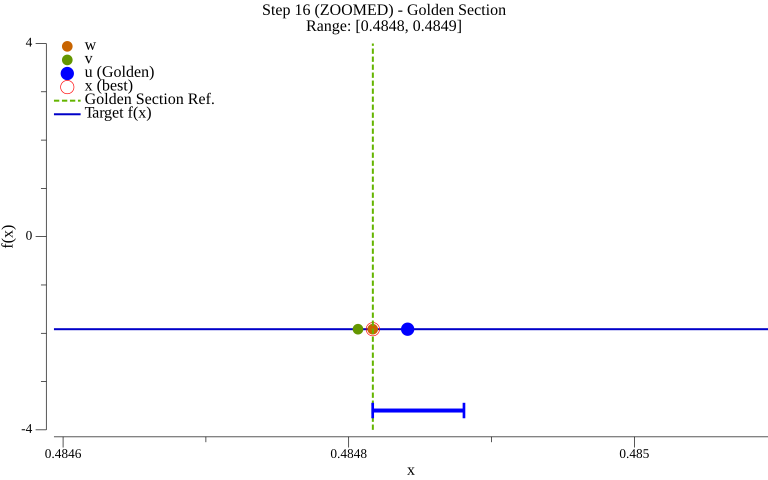
\includegraphics[width=1.0\linewidth]{material/brent/brent-step-16.png}
      \caption{Brent法-16回目}
    \end{minipage}
  \end{figure}
  \begin{figure}[H]
    \begin{minipage}[b]{0.48\linewidth}
      \centering
      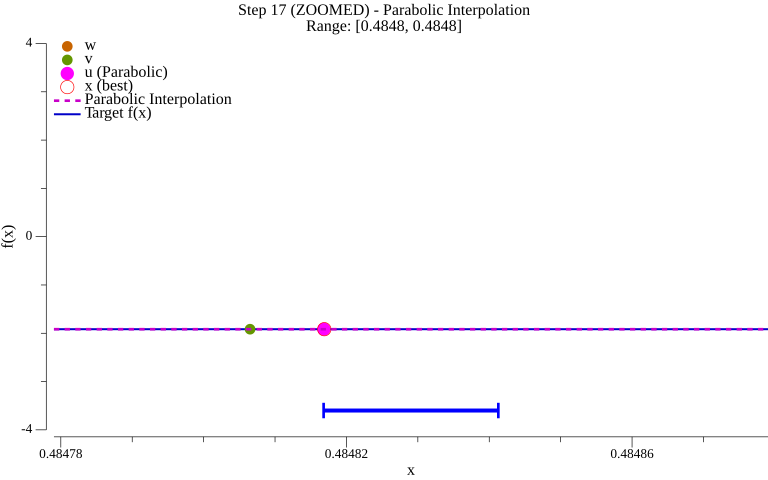
\includegraphics[width=1.0\linewidth]{material/brent/brent-step-17.png}
      \caption{Brent法-17回目}
    \end{minipage}
    \hfill
    \begin{minipage}[b]{0.48\linewidth}
      \centering
      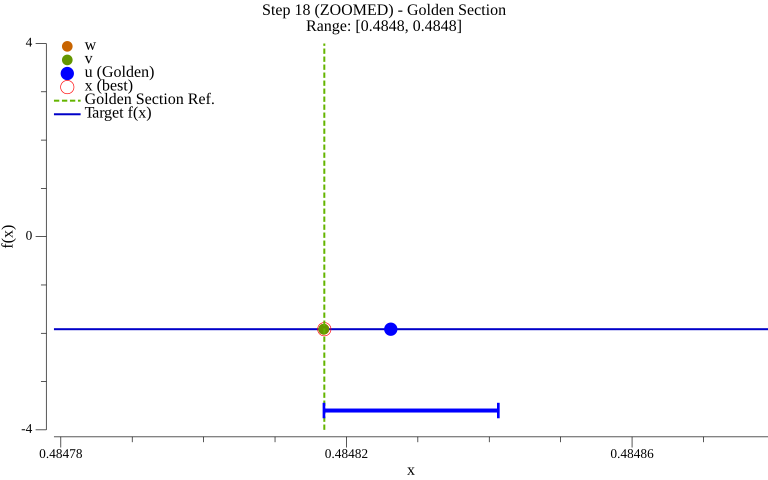
\includegraphics[width=1.0\linewidth]{material/brent/brent-step-18.png}
      \caption{Brent法-18回目}
    \end{minipage}
  \end{figure}
  \begin{figure}[H]
    \begin{minipage}[b]{0.48\linewidth}
      \centering
      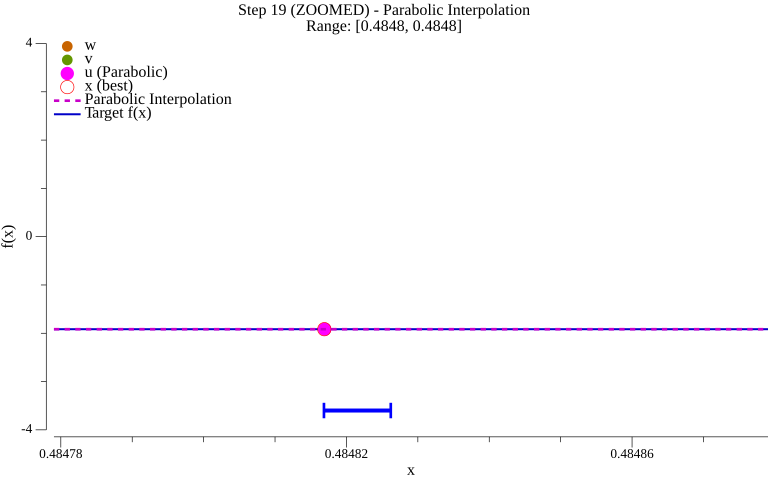
\includegraphics[width=1.0\linewidth]{material/brent/brent-step-19.png}
      \caption{Brent法-19回目}
    \end{minipage}
  \end{figure}
  \begin{figure}[H]
    \centering
    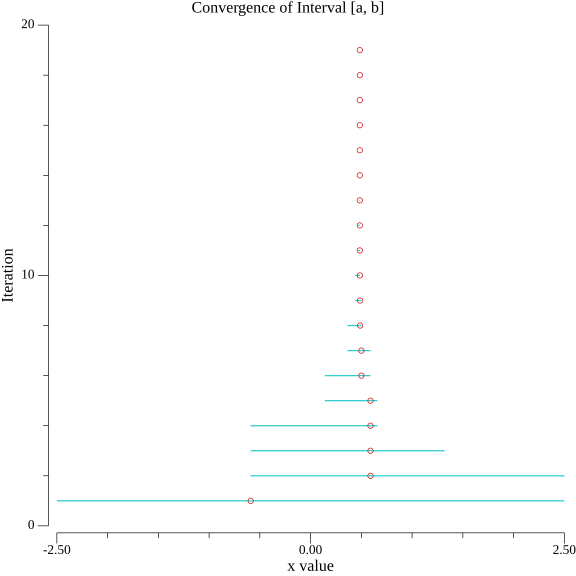
\includegraphics[width=0.7\linewidth]{material/brent/brent-interval.png}
    \caption{Brent法: 探索区間の収束推移}
  \end{figure}


\newpage  %% 改ページ ==================================================